% Chapter Template

\chapter{Results and Analysis} % Main chapter title

\label{c5} % Change X to a consecutive number; for referencing this chapter elsewhere, use \ref{ChapterX}


\section{Results and Analysis}

\subsection{Quantitative Analysis}



\begin{table}[!p]
    \setlength{\tabcolsep}{3pt}
 {\renewcommand{\arraystretch}{1}%
    \caption{Performances of traditional DL models and both proposed models(i.e,  GRU-CNN(proposed-1)) and RB-GRU-CNN(proposed-2)) based on RMSE,  MSE,  MAE and MAPE measures over PTB diagnostic ECG datasets.}
    \label{tab:error_metrics}
    \begin{tabular}{p{0.08\linewidth}cccccccc}
        \toprule
        Error Metric & Dataset & CNN & RNN & LSTM & GRU & BiLSTM & PRO-1 & PRO-2 \\
        \midrule
        \multirow{9}{*}{RMSE} \\
        & D1 & 0.02511 & 0.029045 & 0.02845 & 0.023255 & 0.026725 & 0.017375 & 0.017246 \\
        & D2 & 0.048335 & 0.05851 & 0.033775 & 0.044645 & 0.054565 & 0.016211 & 0.01425 \\
        & D3 & 0.07086 & 0.07155 & 0.07388 & 0.069305 & 0.08139 & 0.04781 & 0.04211\\
        & D4 & 0.053515 & 0.05766 & 0.054275 & 0.051595 & 0.05713 & 0.048195 & 0.040361\\
        & D5 & 0.04291 & 0.02836 & 0.02967 & 0.07155 & 0.07086 & 0.02017 & 0.02\\
        & Mean & 0.048146 & 0.049025 & 0.04401 & 0.05207 & 0.058134 & 0.0299522 & 0.0267934 \\
        \midrule
        \multirow{9}{*}{MSE}\\
        & D1 & 0.000625 & 0.000905 & 0.00085 & 0.000555 & 0.00074 & 0.000315 & 0.000286 \\
        & D2 & 0.00236 & 0.003575 & 0.00118 & 0.002035 & 0.006135 & 0.000315 & 0.00029\\
        & D3 & 0.00505  & 0.00577 & 0.005465 & 0.00483 & 0.00662 & 0.002345 & 0.00219 \\
        & D4 & 0.002925 & 0.00359 & 0.002965 & 0.002685 & 0.00328 & 0.002335 & 0.00202 \\
        & D5 & 0.00204 & 0.00082 & 0.00089 & 0.00577 & 0.00505 & 0.00042 & 0.00031 \\
        & Mean & 0.0026 & 0.002932 & 0.00227 & 0.003175 & 0.004365 & 0.001146 & 0.0010192 \\
        \midrule
        \multirow{9}{*}{MAE}\\
        & D1 & 0.011715 & 0.01838 & 0.01557 & 0.012045 & 0.01579 & 0.00956 & 0.00852 \\
        & D2 & 0.03676 & 0.04618 & 0.01851 & 0.03445 & 0.0415 & 0.00811 & 0.0072 \\
        & D3 & 0.04694 & 0.044345 & 0.048095 & 0.043585 & 0.0491 & 0.03033 & 0.02318 \\
        & D4 & 0.035295 & 0.03525 & 0.03449 & 0.032885 & 0.034545 & 0.03131 & 0.02336 \\
        & D5  & 0.02873 & 0.018095 & 0.018915 & 0.044345 & 0.04694 & 0.011685 & 0.0045 \\
        & Mean & 0.031888 & 0.03245 & 0.027116 & 0.033462 & 0.037575 & 0.018199 & 0.013352 \\
        \midrule
        \multirow{9}{*}{MAPE}\\
        & D1 & 5.758535 & 9.3428 & 7.472155 & 5.433125 & 7.69268 & 4.65592 & 3.22098 \\
        & D2 & 6.144505 & 7.40371 & 9.10457 & 5.852235 & 6.849115 & 3.82211 & 3.2145 \\
        & D3 & 9.79425 & 10.242305 & 9.93871 & 9.85453 & 10.8904 & 5.962575 & 4.376 \\
        & D4 & 8.24417 & 9.73791 & 8.29686 & 8.59091 & 9.001425 & 6.950645 & 4.2018 \\
        & D5 & 4.98369 & 8.88995 & 5.698585 & 10.242305 & 9.79425 & 3.14022 & 3.11067 \\
        & Mean & 6.98503 & 9.123335 & 8.102176 & 7.994621 & 8.845574 & 4.906294 & 3.62479 \\
       
        \bottomrule
    \end{tabular}}
\end{table}

\begin{table}[!h]
\setlength{\tabcolsep}{3pt}
 {\renewcommand{\arraystretch}{1}%
    \caption{Percentage improvement over traditional models based on proposed-1 GRU-CNN model for RMSE,  MSE,  MAE and MAPE measures.}
    \label{tab:error_metrics}
    \begin{tabular}{ccccccc}
        \toprule
        Error Metric & Dataset & \%imp CNN & \%imp RNN & \%imp LSTM & 
        \%imp GRU & \%imp BiLSTM \\
        \midrule
        \multirow{7}{*}{RMSE} \\
        & D1 & 30.80\% & 40.17\% & 38.92\% & 25.28\% & 34.98\% \\
        & D2 & 66.46\% & 72.29\% & 52\% & 52\% & 70.29\% \\
        & D3 & 32.52\% & 33.17\% & 35.28\% & 31.01\% & 41.25\% \\
        & D4 & 9.94\% & 16.41\% & 11.20\% & 6.58\% & 15.63\%\\
        & D5 & 52.99\% & 28.87\% & 32\% & 71.80\% & 71.53\%\\
        & Mean & 38.54\% & 38.18\% & 33.88\% & 37.33\% & 46.74\%\\
        \midrule
        \multirow{7}{*}{MSE}\\
        & D1 & 49.60\% & 65.19\% & 62.94\% & 43.24\% & 57.43\%\\
        & D2 & 86.65\% & 91.18\% & 73.30\% & 84.52\% & 94.86\%\\
        & D3 & 53.56\%  & 59.35\% & 57.09\% & 51.44\% & 64.57\%\\
        & D4 & 20.17\% & 34.95\% & 21.24\% & 13.03\% & 28.81\%\\
        & D5 & 79.41\% & 48.78\% & 52.80\% & 92.72\% & 91.63\%\\
        & Mean & 57.88\% & 59.89\% & 53.47\% & 56.99\% & 67.46\%\\
        \midrule
        \multirow{7}{*}{MAE}\\
        & D1 & 18.39\% & 47.98\% & 38.59\% & 20.63\% & 39.45\%\\
        & D2 & 77.93\% & 82.43\% & 56.18\% & 76.45\% & 80.45\%\\
        & D3 & 35.38\% & 31.60\% & 36.93\% & 30.41\% & 38.22\%\\
        & D4 & 11.29\% & 11.17\% & 9.22\% & 4.78\% & 9.36\%\\
        & D5  & 59.32\% & 35.42\% & 38.22\% & 73.64\% & 75.10\%\\
        & Mean & 40.46\% & 41.72\% & 35.83\% & 41.18\% & 48.52\%\\
        \midrule
        \multirow{7}{*}{MAPE}\\
        & D1 & 19.14\% & 50.16\% & 37.68\% & 14.30\% & 39.47\%\\
        & D2 & 37.79\% & 48.37\% & 58.01\% & 34.68\% & 44.19\%\\
        & D3 & 39.12\% & 41.78\% & 40\% & 39.49\% & 45.24\%\\
        & D4 & 15.69\% & 28.62\% & 16.22\% & 19.09\% & 22.78\%\\
        & D5 & 36.99\% & 64.67\% & 44.89\% & 69.34\% & 67.93\%\\
        & Mean & 29.75\% & 46.72\% & 39.36\% & 35.38\% & 43.92\%\\ 
        \bottomrule
    \end{tabular}}
\end{table}  

It can be seen in Table 1 that on taking four performance metrics the 5 datasets when fed to traditional DL models and compared with proposed-1,  turns out proposed-1 is outperforming implemented traditional models. Proposed-1 is giving least RMSE compared to traditional DL models. Proposed-1(GRU-CNN) on all 5 datasets gave a mean value of RMSE 0.0299522 . A major \% improvement in proposed-1 with respect to traditional DL models can be seen in Table 2 where models CNN,  RNN,  LSTM,  GRU and BiLSTM shown a percentage improvement of 38.54\%,  38.18\%,  33.88\%,  37.33\% and 46.74\% respectively,  which are mean values of \% improvement in RMSE corresponding to datasets with respect to proposed-1 model. Quantitatively proposed-2 is giving less RMSE than proposed-1,  for the model proposed-2 on all 5 datasets a mean value of RMSE 0.0267934 is achieved hence,  it can be concluded that proposed-2 is better than proposed-1 since RMSE of proposed-2 is less than RMSE of proposed-1. 

Similarly,  from Table 1, it can be observed that  Proposed-1 is giving least MSE compared to traditional DL models. Proposed-1 on all 5 datasets gave a mean value of MSE 0.001146 . A major \% improvement in proposed-1 with respect to traditional DL models can be seen in Table 2 where models CNN,  RNN,  LSTM,  GRU and BiLSTM shown a percentage improvement of 57.88\%,  59.89\%,  53.47\%,  56.99\% and 67.46\% respectively,  which are mean values of \% improvement in MSE corresponding to datasets with respect to proposed-1 model. Quantitatively proposed-2 is giving less MSE than proposed-1,  for the model proposed-2 on all 5 datasets a mean value of MSE 0.0010192 is achieved hence,  it can be concluded that proposed-2 is better than proposed-1 since,  MSE of proposed-2 is less than MSE of proposed-1. 

Again,  from Table 1 it can be observed that  Proposed-1 is giving least MAE compared to traditional DL models. Proposed-1 on all 5 datasets gave a mean value of MAE 0.018199 . A major \% improvement in proposed-1 with respect to traditional DL models can be seen in Table 2 where models CNN,  RNN,  LSTM,  GRU and BiLSTM shown a percentage improvement of 40.46\%,  41.72\%,  35.83\%,  41.18\% and 48.52\% respectively,  which are mean values of \% improvement in MAE corresponding to datasets with respect to proposed-1 model. Quantitatively proposed-2 is giving less MAE than proposed-1,  for the model proposed-2 on all 5 datasets a mean value of MAE 0.013352 is achieved Hence,  it can be concluded that proposed-2 is better than proposed-1 since MAE of proposed-2 is less than MAE of proposed-1.

At last,  from Table 1 it can be observed that  Proposed-1 is giving least MAPE compared to traditional DL models. Proposed-1 on all 5 datasets gave a mean value of MAPE 4.906294 . A major \% improvement in proposed-1 with respect to traditional DL models can be seen in Table 2 where models CNN,  RNN,  LSTM,  GRU and BiLSTM shown a percentage improvement of 29.75\%,  46.72\%,  39.36\%,  35.38\% and 43.92\% respectively,  which are mean values of \% improvement in MAPE corresponding to datasets with respect to proposed-1 model. Quantitatively proposed-2 is giving less MAPE than proposed-1,  for the model proposed-2 on all 5 datasets a mean value of MAPE 3.62479 is achieved hence,  it can be concluded that proposed-2 is better than proposed-1 since MAPE of proposed-2 is less than MAPE of proposed-1.
 \begin{figure*}[h!]
   \centering
   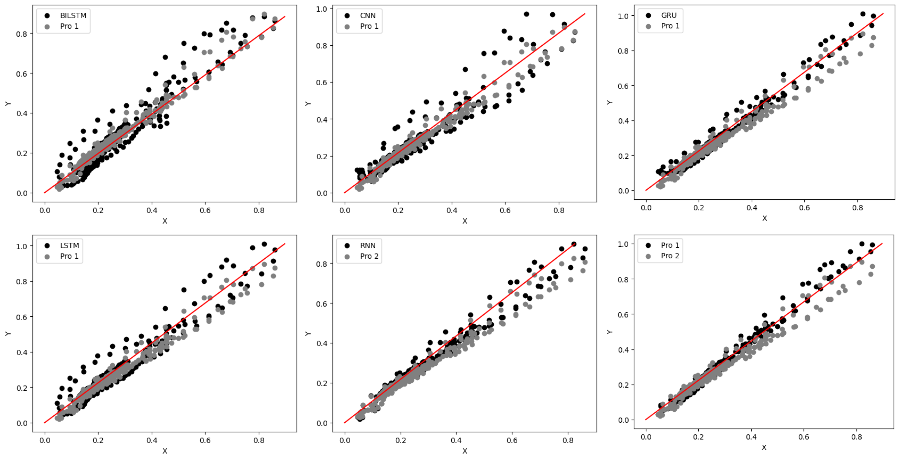
\includegraphics[scale=.5]{d1_sp.drawio.png}
     %\captionsetup{justification=centering, margin=2cm}
    \caption{Scatter plots of proposed GRU-CNN(pro-1) with stand alone DL models along with proposed-2 RB-GRU-CNN(pro-2), where x-axis \& y-axis represent the predictions of models and original test data D1.}
    \label{Fig:6}
   \end{figure*}
   \begin{figure*}[h!]
    \centering
     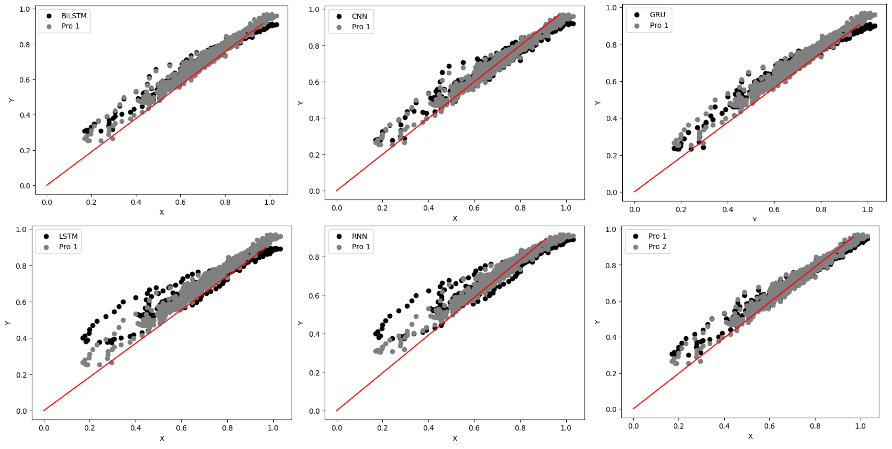
\includegraphics[scale=.5]{d2_sp.drawio.png}
     \caption{Scatter plots of proposed GRU-CNN(pro-1) with stand alone DL models along with proposed-2 RB-GRU-CNN(pro-2), where x-axis \& y-axis represent the predictions of models and original test data D2.}
     \label{Fig:7}
  \end{figure*}
  \begin{figure*}[h!]
     \centering
     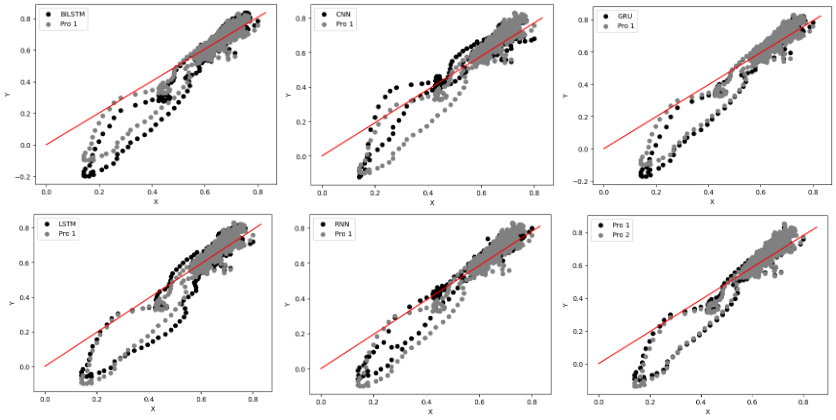
\includegraphics[scale=.5]{d3_sp.drawio.png}
     \caption{Scatter plots of proposed GRU-CNN(pro-1) with stand alone DL models along with proposed-2 RB-GRU-CNN(pro-2), where x-axis \& y-axis represent the predictions of models and original test data D3.}
     \label{Fig:8}
   \end{figure*}
   \begin{figure*}[h!]
    \centering
     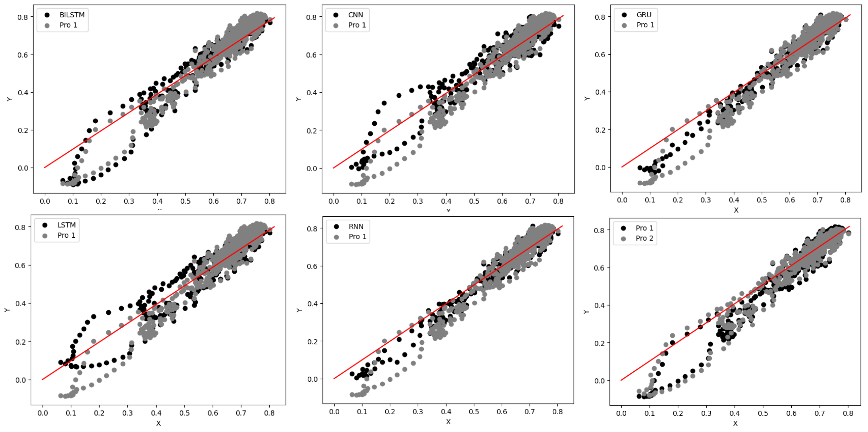
\includegraphics[scale=.5]{d4_sp.drawio.png}
     \caption{Scatter plots of proposed GRU-CNN(pro-1) with stand alone DL models along with proposed-2 RB-GRU-CNN(pro-2), where x-axis \& y-axis represent the predictions of models and original test data D4.}
     \label{Fig:9}
   \end{figure*}
   \begin{figure}[h!]
    \centering
     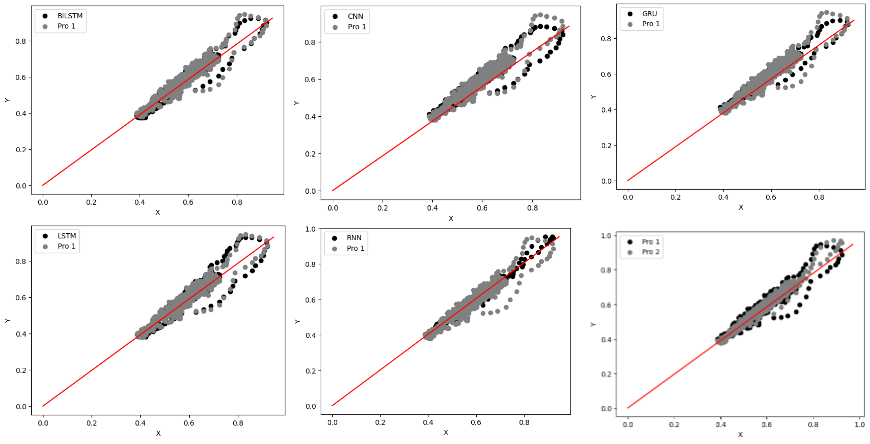
\includegraphics[scale=.5]{d5_sp.drawio.png}
     \caption{Scatter plots of proposed GRU-CNN(pro-1) with stand alone DL models along with proposed-2 RB-GRU-CNN(pro-2), where x-axis \& y-axis represent the predictions of models and original test data D5.}
     \label{Fig:10}
   \end{figure}

   \begin{figure*}[h!]
    \centering
     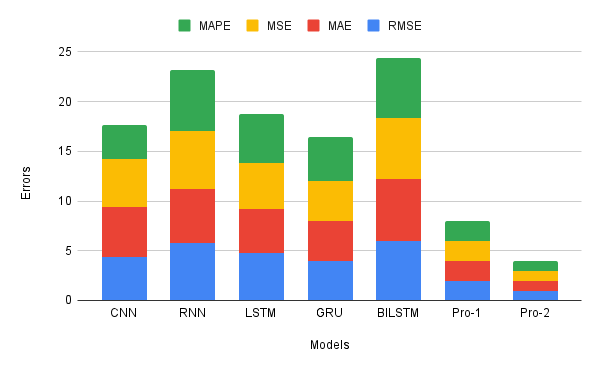
\includegraphics[scale=.6]{aggregator.png}
     \caption{Aggregate measures comparison of traditional models and proposed (pro-1 \& pro-2) models.}
     \label{Fig:13}
   \end{figure*} 
\subsection{Graphical Analysis}
 \begin{figure*}[h!]
    \centering
    \subfigure{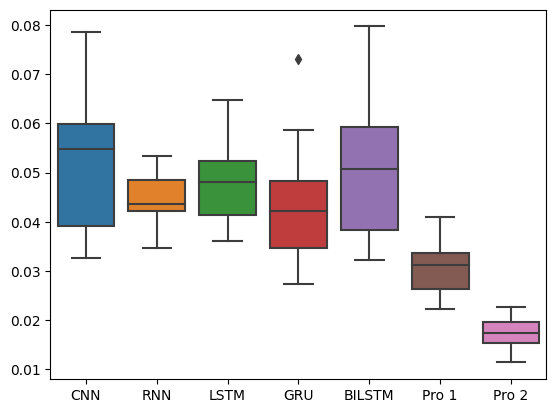
\includegraphics[scale=0.5]{d1rmse}}
    \subfigure{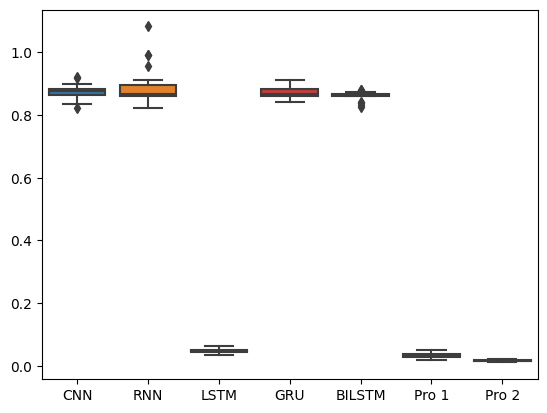
\includegraphics[scale=0.5]{D2_RMSE}}
    \subfigure{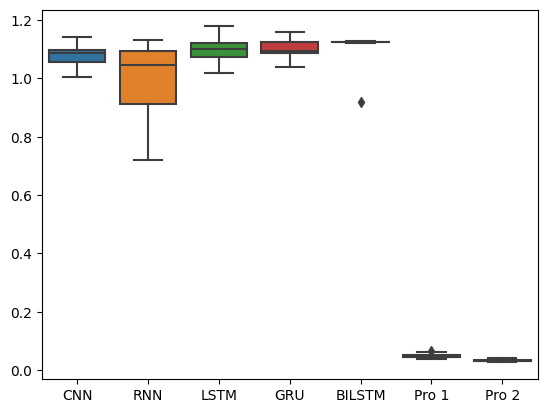
\includegraphics[scale=0.5]{D3_RMSE}}
    \subfigure{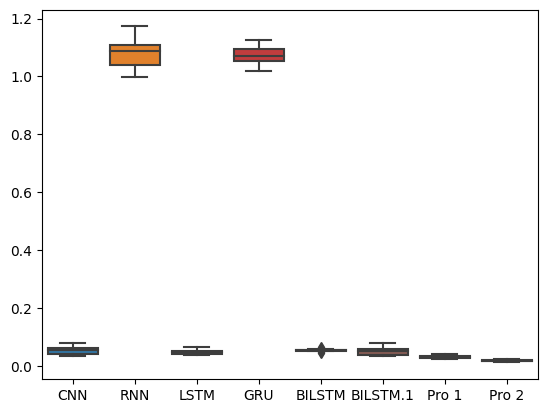
\includegraphics[scale=0.5]{d4_rmse}}
    \subfigure{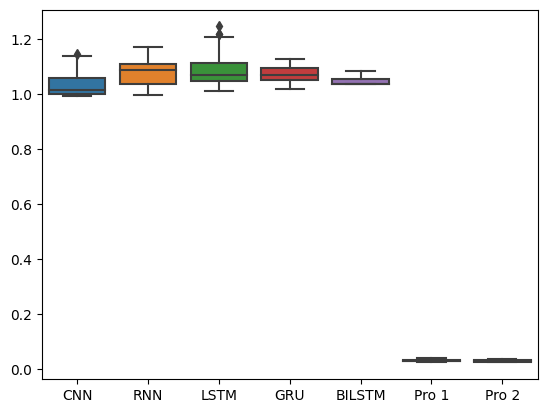
\includegraphics[scale=0.5]{D5_RMSE}}
    \caption{RMSE (performance box-plots) of basic DL models with proposed hybrid models (pro-1 \& pro-2).}
    \label{Fig:14}
  \end{figure*}

  \begin{figure*}[h!]
    \centering
    \subfigure{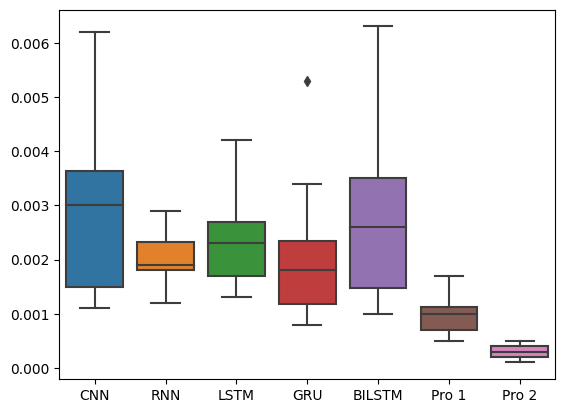
\includegraphics[scale=0.5]{d1_mse}}
    \subfigure{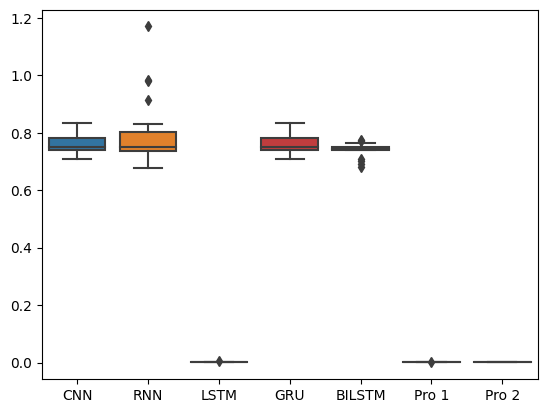
\includegraphics[scale=0.5]{D2_MSE}}
    \subfigure{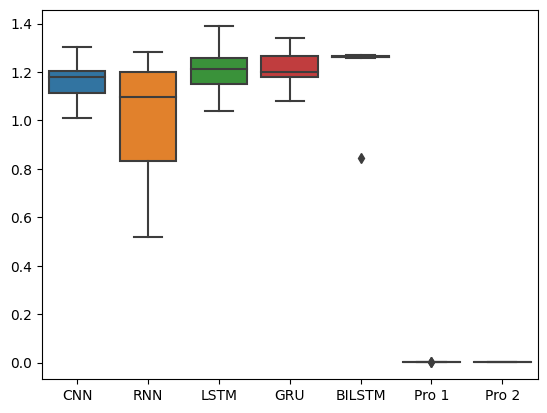
\includegraphics[scale=0.5]{D3_MSE}}
    \subfigure{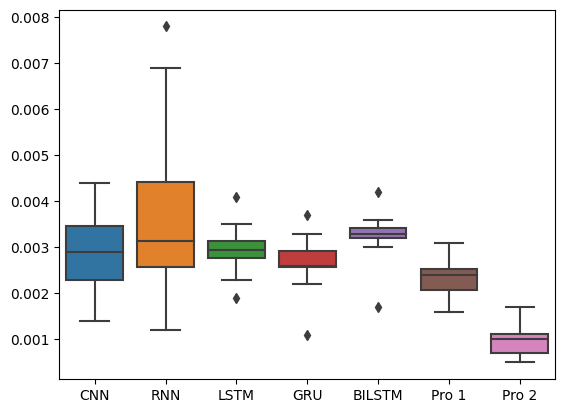
\includegraphics[scale=0.5]{d4_mse}}
    \subfigure{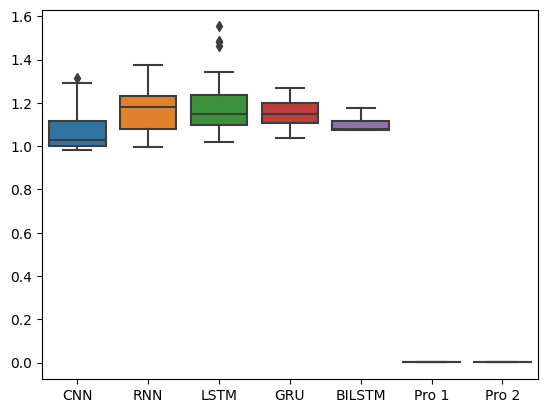
\includegraphics[scale=0.5]{D5_MSE}}
    \caption{MSE (performance box-plots) of basic DL models with proposed hybrid models (pro-1 \& pro-2).}
    \label{Fig:15}
  \end{figure*}

  \begin{figure*}[h!]
   \centering
    \subfigure{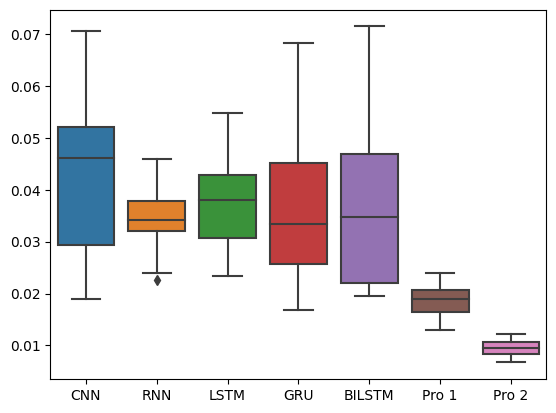
\includegraphics[scale=0.5]{d1_mae}} 
    \subfigure{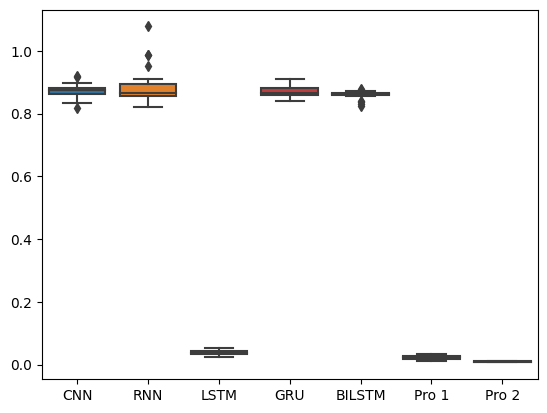
\includegraphics[scale=0.5]{D2_MAE}}
    \subfigure{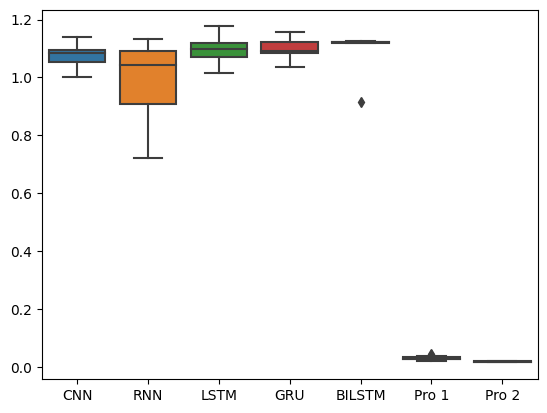
\includegraphics[scale=0.5]{D3_MAE}}
    \subfigure{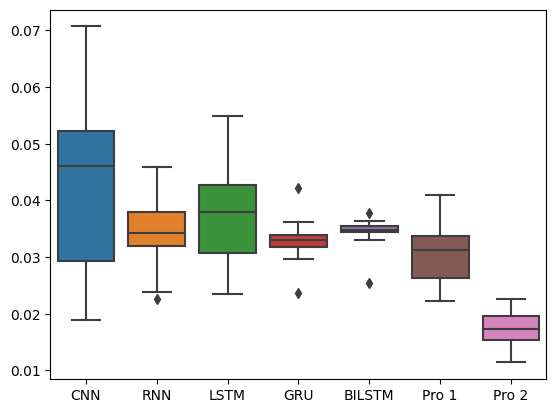
\includegraphics[scale=0.5]{d4_mae}}
    \subfigure{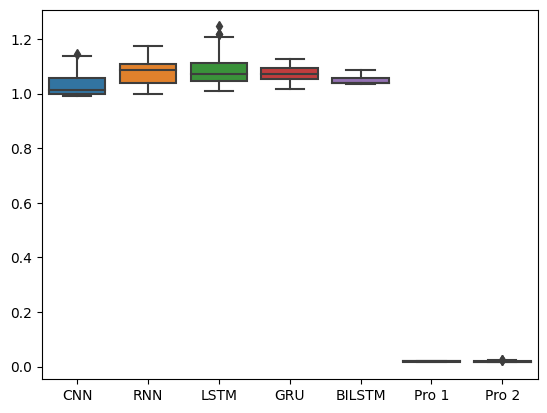
\includegraphics[scale=0.5]{D5_MAE}}
    \caption{MAE (performance box-plots) of basic DL models with proposed hybrid models (pro-1 \& pro-2).}
    \label{Fig:16}
  \end{figure*}
  \begin{figure*}[h!]
    \centering
    \subfigure{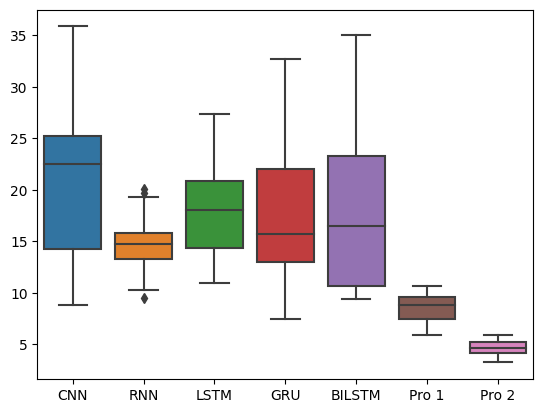
\includegraphics[scale=0.5]{d1_mape}}
    \subfigure{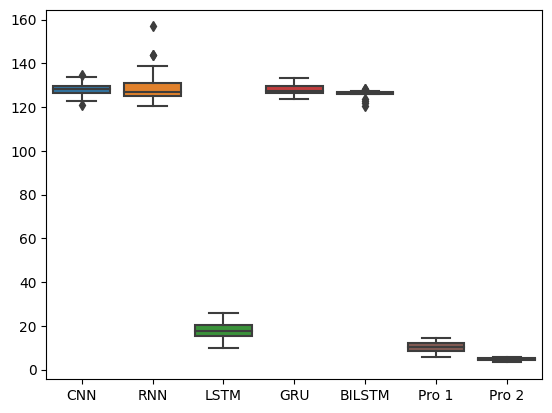
\includegraphics[scale=0.5]{D2_MAPE}}
    \subfigure{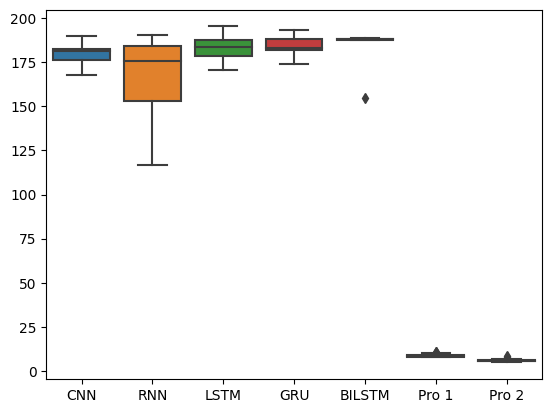
\includegraphics[scale=0.5]{D3_MAPE}}
    \subfigure{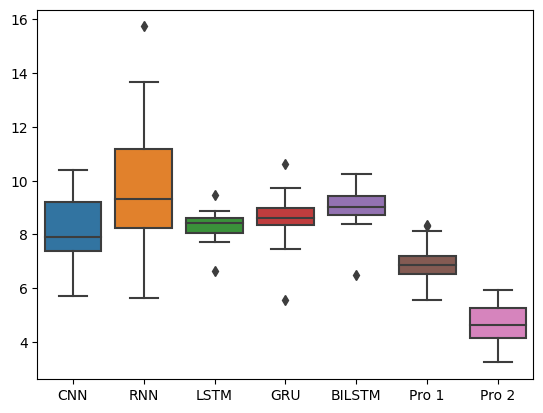
\includegraphics[scale=0.5]{d4_mape}} 
    \subfigure{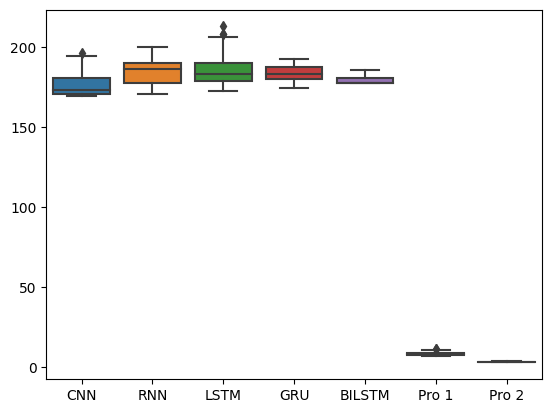
\includegraphics[scale=0.5]{D5_MAPE}}
    \caption{MAPE (performance box-plots) of basic DL models with proposed hybrid models (pro-1 \& pro-2).}
    \label{Fig:17}
  \end{figure*}
In this section graphical analysis of our experiments is shown. Overlaying the scatterplot is a line of regression with a distinct 45-degree angle. The angle indicates that there is a high positive correlation between the two variables,  implying a linear relationship. Two more regression lines are visible on the scatterplot upon closer scrutiny. One of these lines closely follows the general trend of the data points,  with a relatively limited deviation off the line. This indicates a good fit for the data and a high prediction power for the model it represents. Although it still follows the main trend,  the other regression line deviates further from the scatterplot's points. This line clearly has a larger range of data points surrounding it. This indicates a poorer fit than the first model. When the two models are compared,  it is evident that the first,  with its narrower spread and greater alignment to the data points,  produces more accurate results. In Figure 8 on dataset D1 proposed-1(pro-1) can be seen scattered and overlapping the traditional DL models and in the last figure proposed-2 is overlapping proposed-1 validating proposed-1 to be outperforming traditional DL models and proposed-2(pro-2) is better than proposed-1. Similarly,  it can be understood for Figure 9,  10,  11 and 12 where predicted dataset belongs to D2,  D3,  D4 and D5. Boxplot has the ability to obtain insights into the distribution of numerical data,  it is one of the best ways to undertake statistical analysis since it gives a compact approach to visualise the spread,  central tendency,  and probable outliers. It can be seen from the plot in Figure 14 all five datasets are analysed on the basis of RMSE,  where traditional models are compared with proposed-1 and proposed-2. Here proposed-2 is better than proposed-1 and traditional DL models are outperformed by the proposed ones. Similarly,  in Figure 15 all five datasets are analysed on the basis of MSE and comparative analysis has outperformed the traditional DL models,  with proposed-2 is better than proposed-1. Again in Figure 16 a comparative analysis on the basis of MAE is observed corresponding to all five datasets,  where proposed-2 is working better than proposed-1 and outperforming the traditional DL models. At last in Figure 17 it can be observed,  analysis of traditional DL models is performed corresponding to five datasets with proposed-1 and proposed-2 on taking MAPE the metric,  where proposed-2 is seen to be working better than proposed-1 and proposed-1 outperforming the rest of the traditional DL models. A summarised analysis can be understood by plot Figure 13 that shows all performance metric to be averaged and plotted against the traditional and proposed models. It can be concluded from the figure that pro-1(proposed-1) is giving minimum error compared to traditional DL models and pro-2(proposed-2) is giving less error than proposed-1 hence, the best among all.
 

\subsection{Statistical Analysis}

In this section Friedman test is used to validate proposed-1 and proposed-2  are better performing models than traditional DL models on the basis of rank,  p-value and holm. A non-parametric statistical test is performed on RMSE,  MSE,  MAE and MAPE achieved by taking the mean of results achieved after 20 iterations of every single model. Table 3 shows non-parametric test results where it can be seen that our proposed-2 giving rank 1 on all the performance measures while,  proposed-1 came to be following rank 2. The null hypothesis is rejected for proposed-1 because of its p-value 0.464214 which is greater than  $\alpha = 0.05$ , 
 which means proposed-1 and proposed-2 have similar performance. However,  based on holm’s procedure the hypothesis of proposed-1 is rejected because its holm’s value is 0.05,  which is equal to hypothesis value. Therefore,  it can be said that the proposed-1 and proposed-2 models are distinct based on holm’s procedure. The values and Ranking are as follows Figure 18:

\begin{figure*}[ht!]
  \centering
   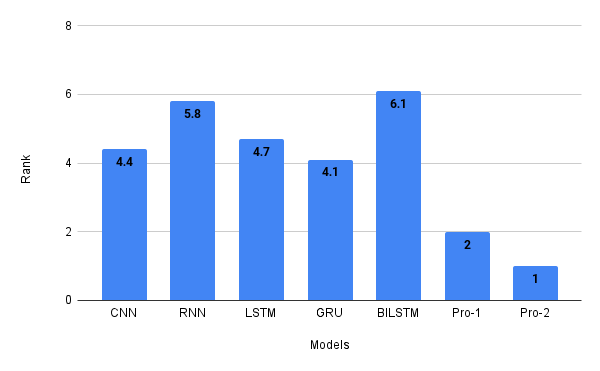
\includegraphics[scale=.7]{rankplot.png}
   \caption{Overall ranking of Traditional models \& Proposed models corresponding to all performance measures.}
 \end{figure*}

\begin{table}[htbp]
\centering
    \setlength{\tabcolsep}{3pt}
 {\renewcommand{\arraystretch}{1}%
    \caption{Non-parametric statistical analysis via Friedman ranking,  p-value \& Holm's procedure over various performance measure as RMSE,  MSE,  MAE and MAPE.}
    \begin{tabular}{cccccc}
        \toprule
        Error Metric & Models & RANK & P-value & Holm \\
        \midrule
        \multirow{5}{*}{RMSE} & CNN & 4.4 & \textbf{0.012827} & \textbf{0.016667} \\
        & RNN & 5.8 & \textbf{0.000443} & \textbf{0.01} \\
        & LSTM & 4.8 & \textbf{0.005414} & \textbf{0.0125} \\
        & GRU & 4 & \textbf{0.028108} & \textbf{0.025} \\
        & BiLSTM & 6 & \textbf{0.000253} & \textbf{0.008333} \\
        & Pro-1 & 2  & 0.464214 & 0.05\\
        & Pro-2 & \textbf{1}  & - & -\\
        \midrule
        \multirow{5}{*}{MSE} & CNN & 4.4 & \textbf{0.012827} & \textbf{0.016667} \\
        & RNN & 5.8 & \textbf{0.000443} & \textbf{0.01} \\
        & LSTM & 4.6 & \textbf{0.008415} & \textbf{0.0125} \\
        & GRU & 4 & \textbf{0.028108} & \textbf{0.025} \\
        & BiLSTM & 6.2 & \textbf{0.000141} & \textbf{0.008333} \\
        & Pro-1 & 2 & 0.464214 & 0.05 \\
        & Pro-2 & \textbf{1}  & - & -\\
        \midrule
        \multirow{5}{*}{MAE} & CNN & 5 & \textbf{0.003415} & \textbf{0.0125} \\
        & RNN & 5.4 & \textbf{0.00128} & \textbf{0.01} \\
        & LSTM & 4.4 & \textbf{0.012827} & \textbf{0.016667} \\
        & GRU & 4 & \textbf{0.028108} & \textbf{0.025} \\
        & BiLSTM & 6.2 & \textbf{0.000141} & \textbf{0.008333} \\
        & Pro-1 & 2 & 0.464214 & 0.05 \\
        & Pro-2 & \textbf{1}  & - & -\\
        \midrule
        \multirow{5}{*}{MAPE} & CNN & 3.4 & \textbf{0.078983} & \textbf{0.025} \\
        & RNN & 6.2 & \textbf{0.000141} & \textbf{0.008333} \\
        & LSTM & 5 & \textbf{0.003415} & \textbf{0.0125} \\
        & GRU & 4.4 & \textbf{0.012827} & \textbf{0.016667} \\
        & BiLSTM & 6 & \textbf{0.000253} & \textbf{0.01} \\
        & Pro-1 & 2 & 0.464214 & 0.05 \\
        & Pro-2 & \textbf{1}  & - & -\\
        \bottomrule
    \end{tabular}}
    
    \label{tab:error_metrics}
\end{table}
